\documentclass[12pt,letterpaper]{article}
\usepackage[utf8]{inputenc}
\usepackage[spanish]{babel}
\usepackage{graphicx}
\usepackage[left=2cm,right=2cm,top=2cm,bottom=2cm]{geometry}
\usepackage{graphicx} % figuras
% \usepackage{subfigure} % subfiguras
\usepackage{float} % para usar [H]
\usepackage{amsmath}
%\usepackage{txfonts}
\usepackage{stackrel} 
\usepackage{multirow}
\usepackage{enumerate} % enumerados
\renewcommand{\labelitemi}{$-$}
\renewcommand{\labelitemii}{$\cdot$}
% \author{}
% \title{Caratula}
\begin{document}

% Fancy Header and Footer
% \usepackage{fancyhdr}
% \pagestyle{fancy}
% \cfoot{}
% \rfoot{\thepage}
%

% \usepackage[hidelinks]{hyperref} % CREA HYPERVINCULOS EN INDICE

% \author{}
\title{Caratula}

\begin{titlepage}
\begin{center}
\large{UNERSIDAD PRIVADA DE TACNA}\\
\vspace*{-0.025in}
\begin{figure}[htb]
\begin{center}

\includegraphics[width=8cm]{./Imagenes/logo}
\end{center}
\end{figure}
\vspace*{0.15in}
INGENIERIA DE SISTEMAS  \\

\vspace*{0.5in}
\begin{large}
TITULO:\\
\end{large}

\vspace*{0.1in}
\begin{Large}
\textbf{INFORME DE LABORATORIO No 03} \\
\end{Large}

\vspace*{0.3in}
\begin{Large}
\textbf{CURSO:} \\
\end{Large}

\vspace*{0.1in}
\begin{large}
BASE DE DATOS II\\
\end{large}

\vspace*{0.3in}
\begin{Large}
\textbf{DOCENTE(ING):} \\
\end{Large}

\vspace*{0.1in}
\begin{large}
 Patrick Cuadros Quiroga\\
\end{large}

\vspace*{0.2in}
\vspace*{0.1in}
\begin{large}
Alumna: \\
\begin{flushleft}
Huallpa Castro Leydi Katherine 		\hfill	(2015053230) \\
\end{flushleft}
\end{large}
\end{center}

\end{titlepage}


\tableofcontents % INDICE
\thispagestyle{empty} % INDICE SIN NUMERO
\newpage
\setcounter{page}{1} % REINICIAR CONTADOR DE PAGINAS DESPUES DEL INDICE

 \section{Actividad No 01 – DESARROLLO1} 
Ejercicio 1  Conectar a datos existentes \\
	\begin{center}
	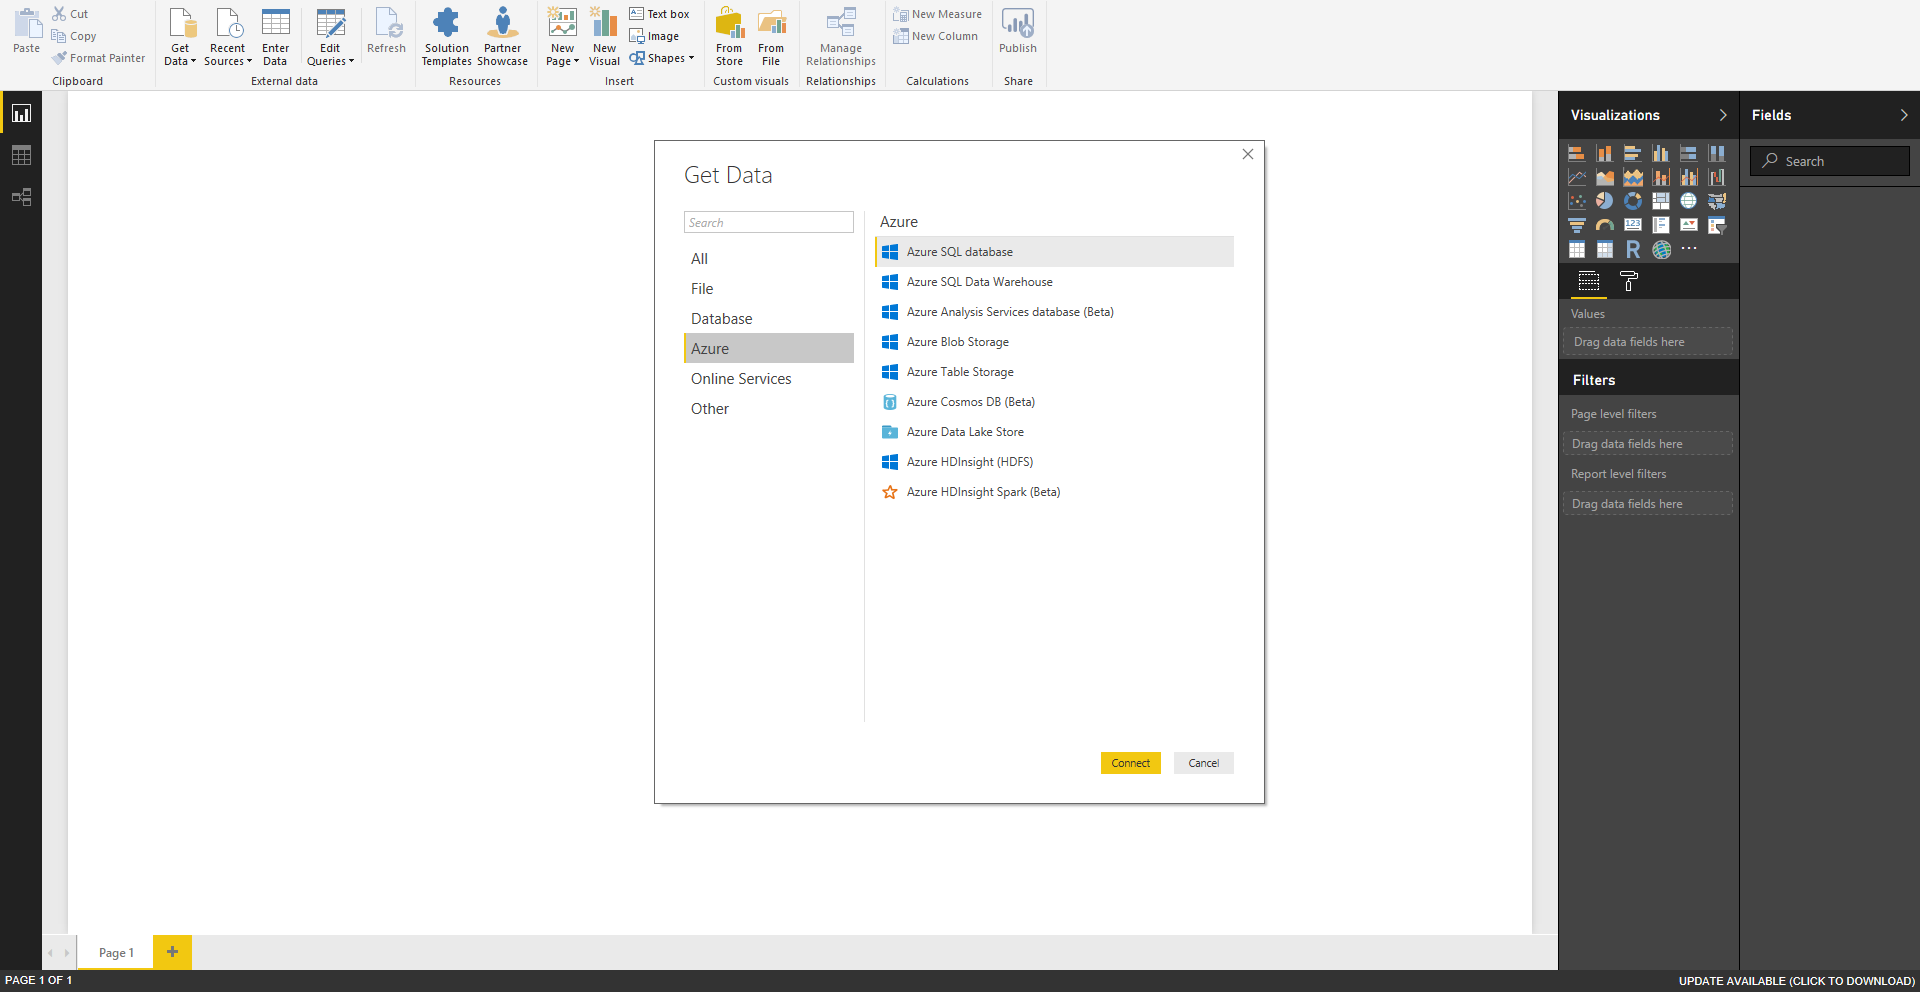
\includegraphics[width=15cm]{./Imagenes/EJER1T1(1)}
	\end{center}	

	\begin{center}
	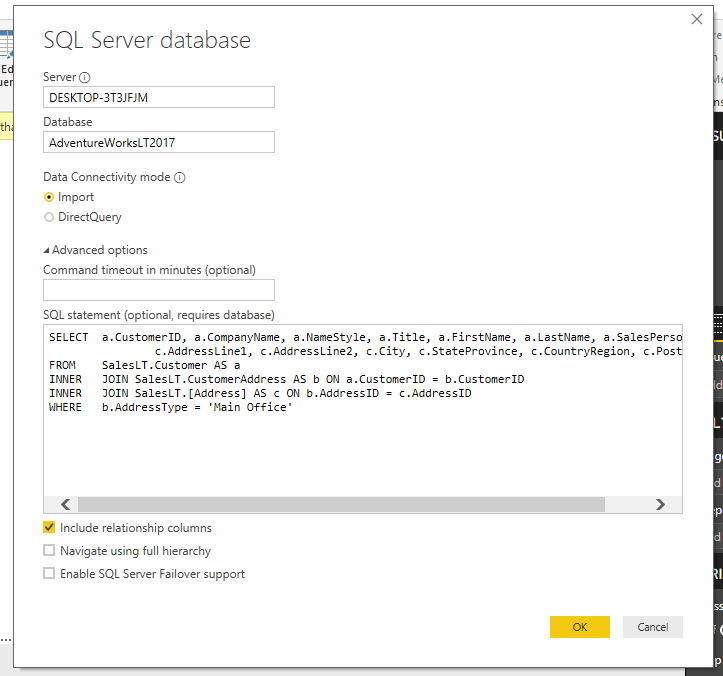
\includegraphics[width=15cm]{./Imagenes/EJER1T1(2)}
	\end{center}	

	\begin{center}
	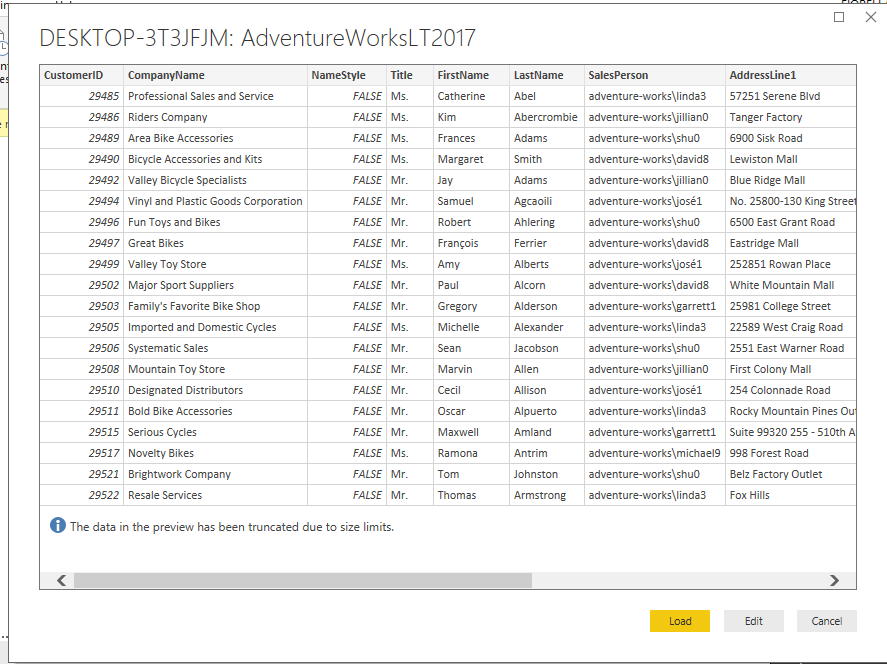
\includegraphics[width=15cm]{./Imagenes/EJER1T1(3)}
	\end{center}	

	\begin{center}
	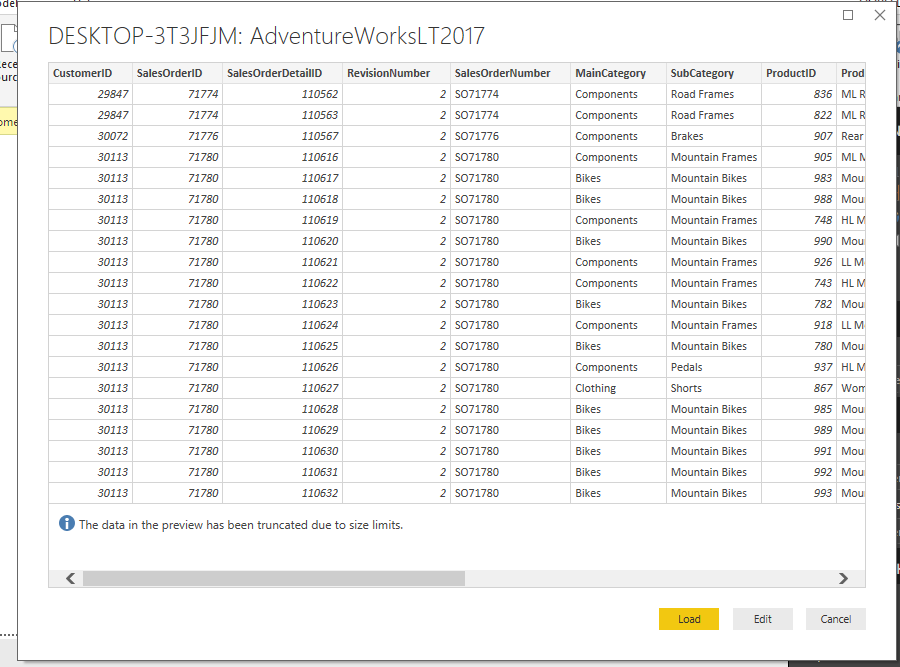
\includegraphics[width=15cm]{./Imagenes/EJER1T1(4)}
	\end{center}	
Ejercicio 2: Shape Data\\
	\begin{center}
	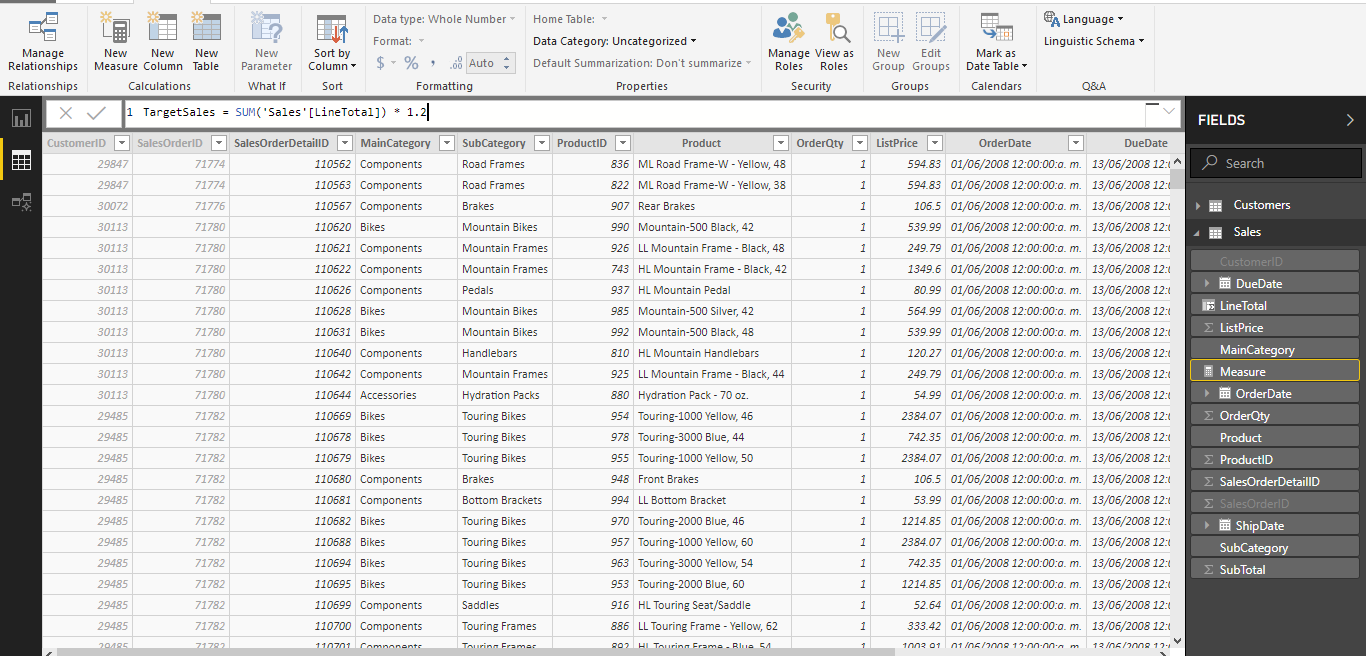
\includegraphics[width=15cm]{./Imagenes/EJER1T2(1)}
	\end{center}	

	\begin{center}
	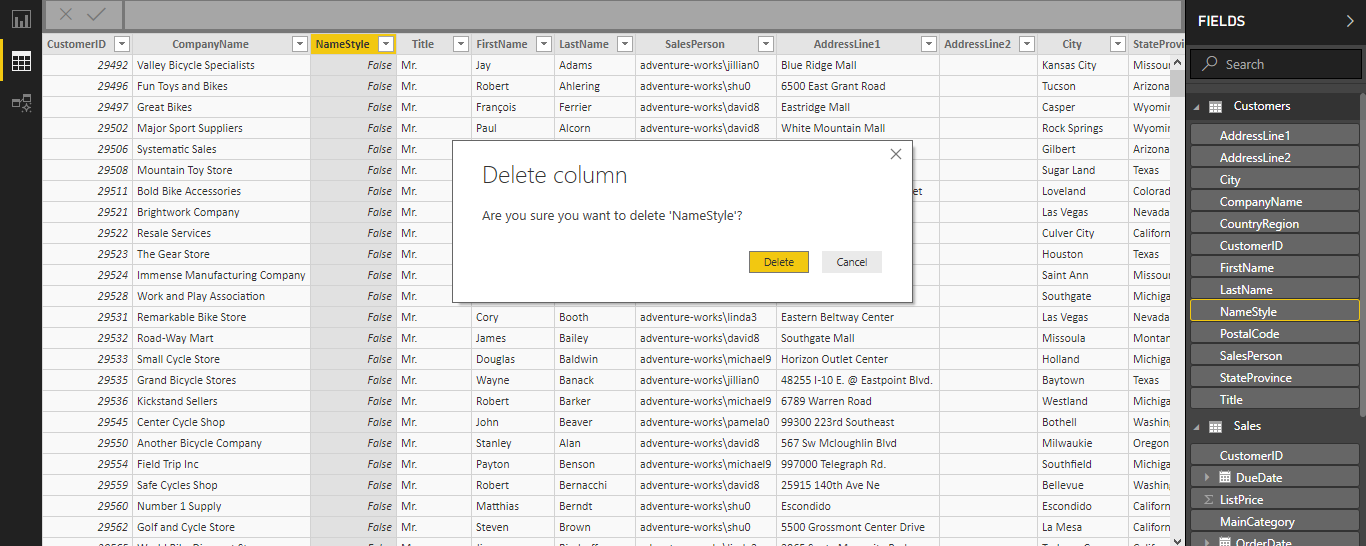
\includegraphics[width=15cm]{./Imagenes/EJER1T2(2)}
	\end{center}	

	\begin{center}
	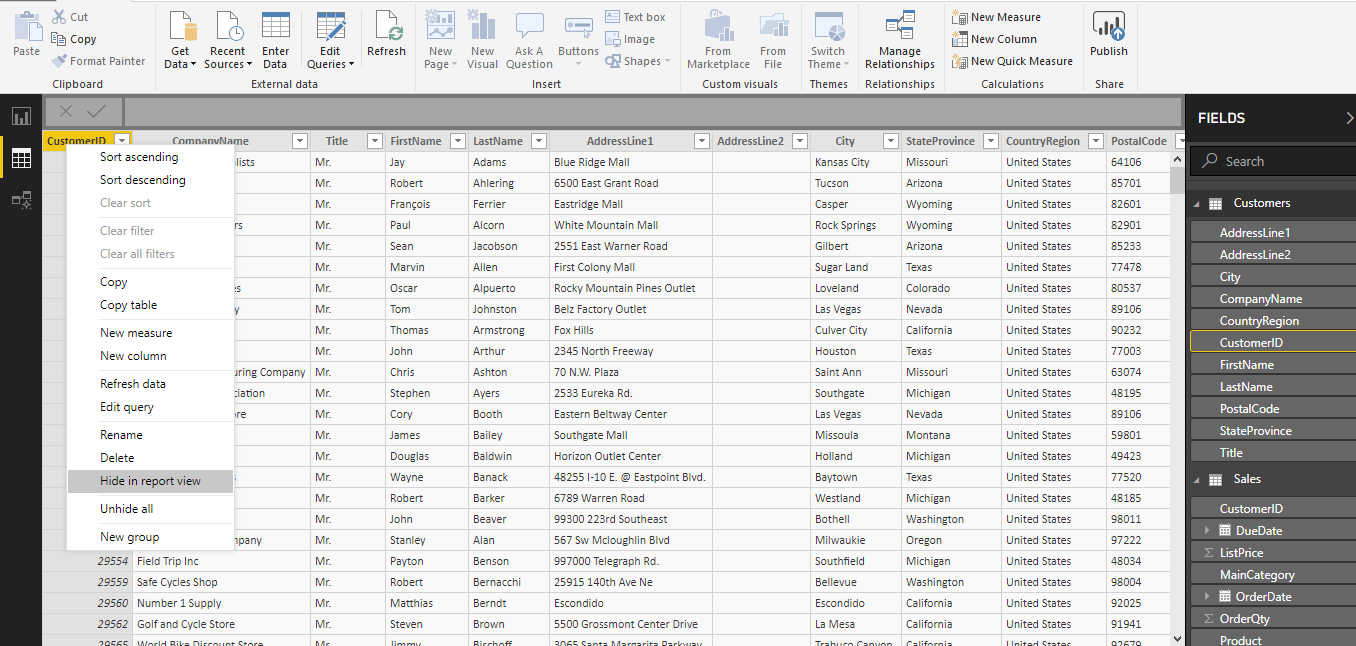
\includegraphics[width=15cm]{./Imagenes/EJER1T2(3)}
	\end{center}	

	\begin{center}
	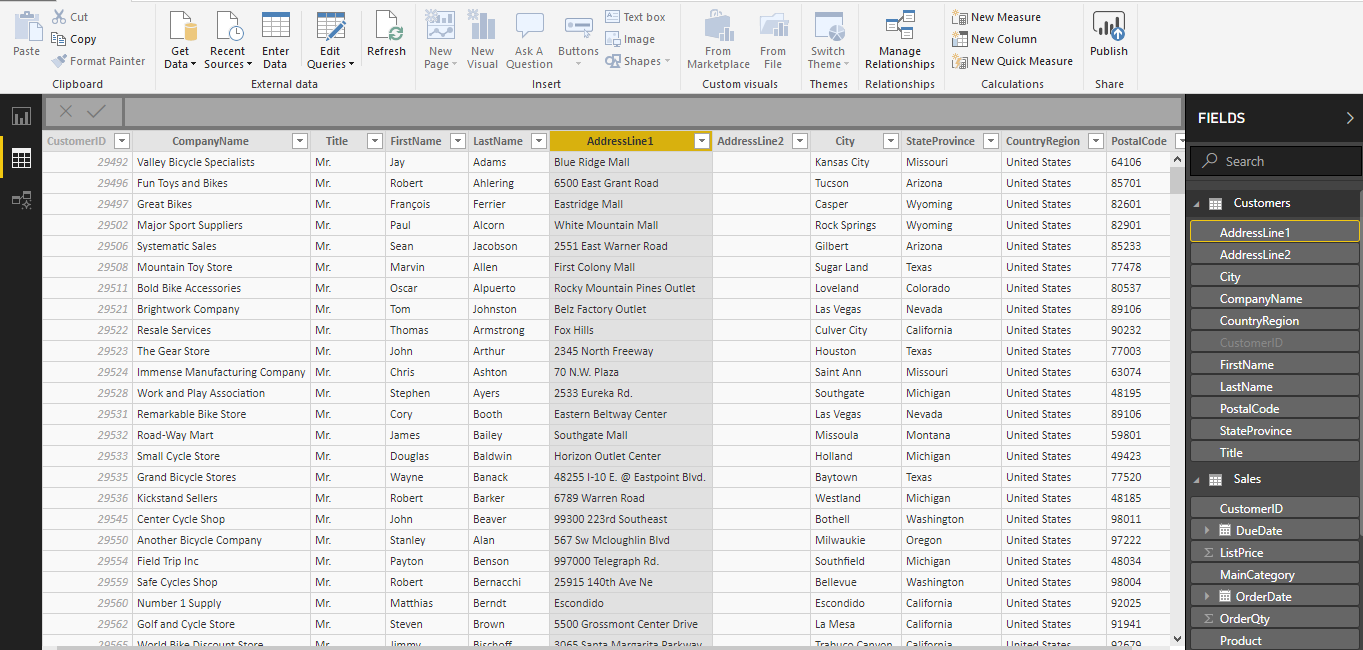
\includegraphics[width=15cm]{./Imagenes/EJER1T2(4)}
	\end{center}	

	\begin{center}
	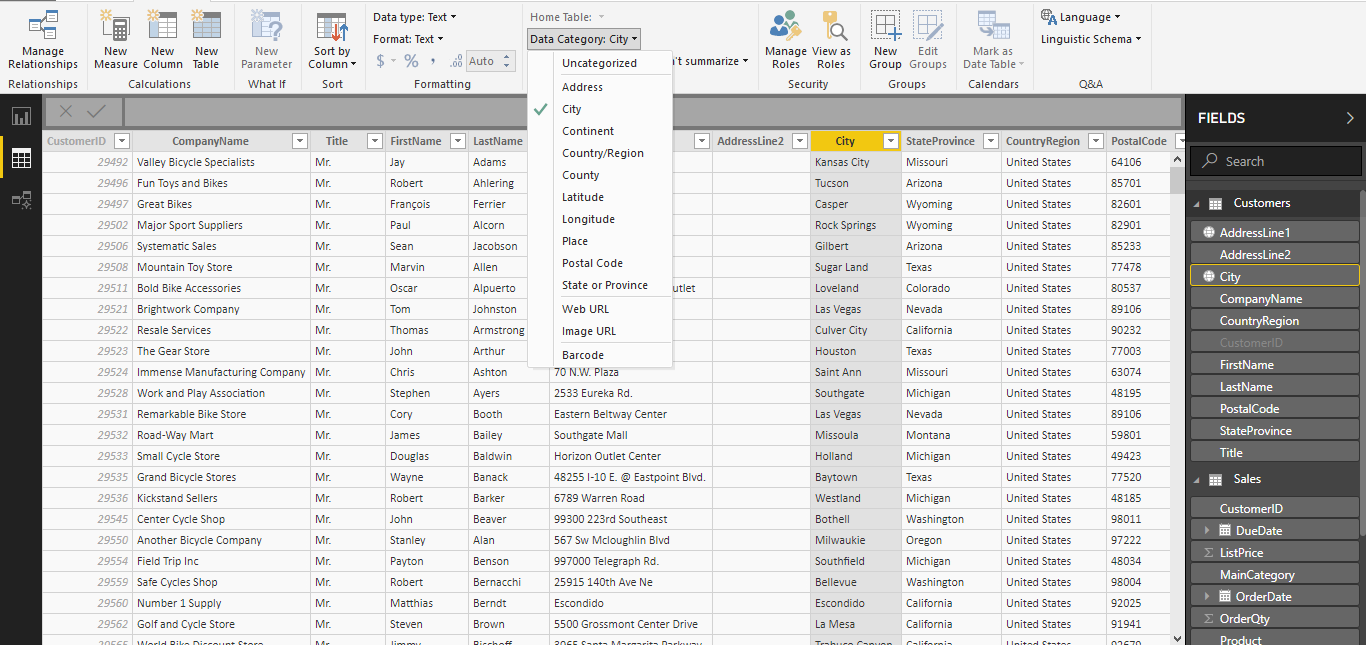
\includegraphics[width=15cm]{./Imagenes/EJER1T2(5)}
	\end{center}	

	\begin{center}
	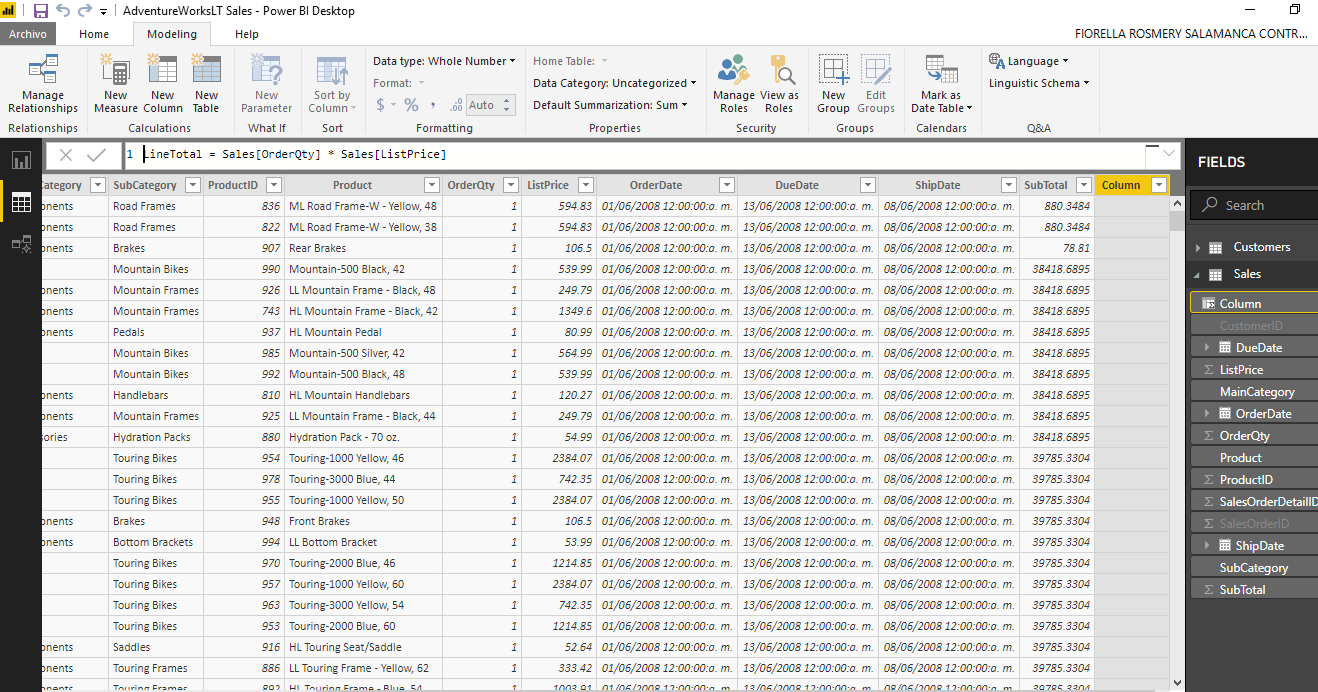
\includegraphics[width=15cm]{./Imagenes/EJER1T2(6)}
	\end{center}	

	\begin{center}
	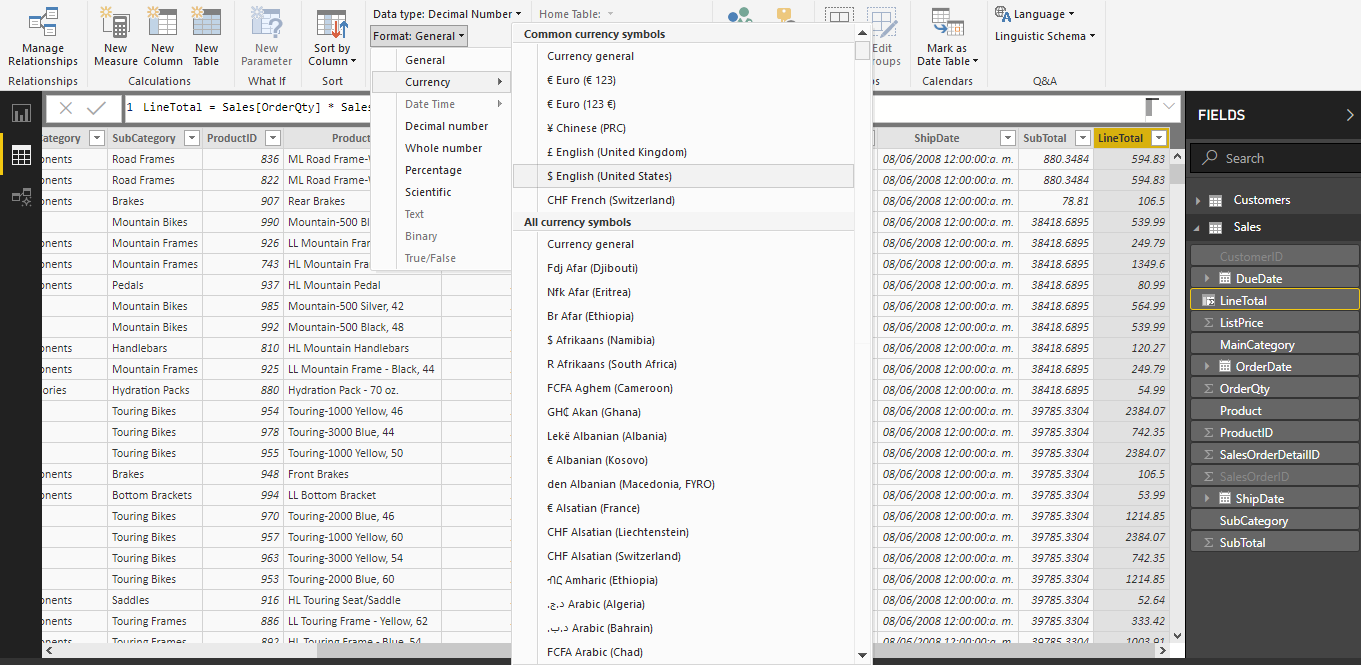
\includegraphics[width=15cm]{./Imagenes/EJER1T2(7)}
	\end{center}	

	\begin{center}
	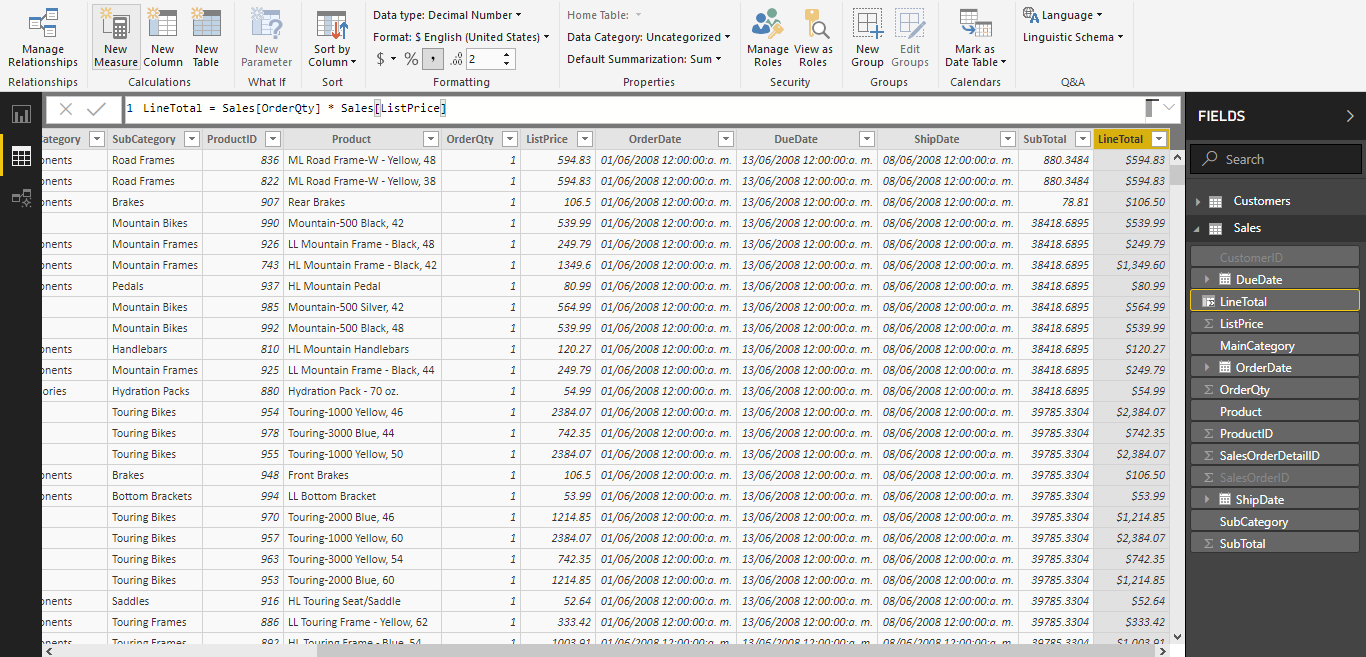
\includegraphics[width=15cm]{./Imagenes/EJER1T2(8)}
	\end{center}	
Ejercicio 3: Combine Data\\
	\begin{center}
	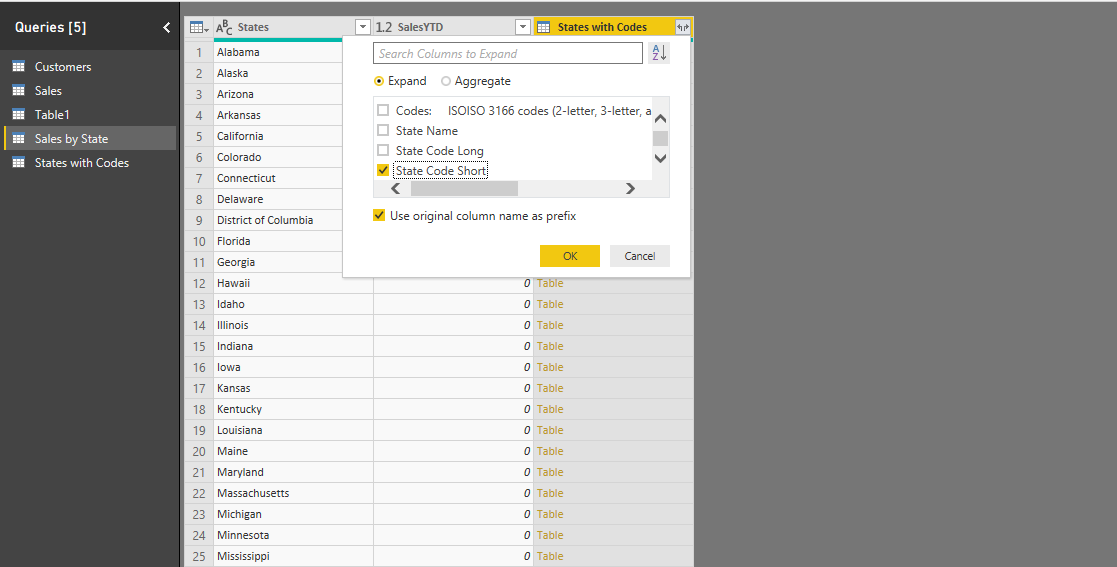
\includegraphics[width=15cm]{./Imagenes/EJER1T3(1)}
	\end{center}	

	\begin{center}
	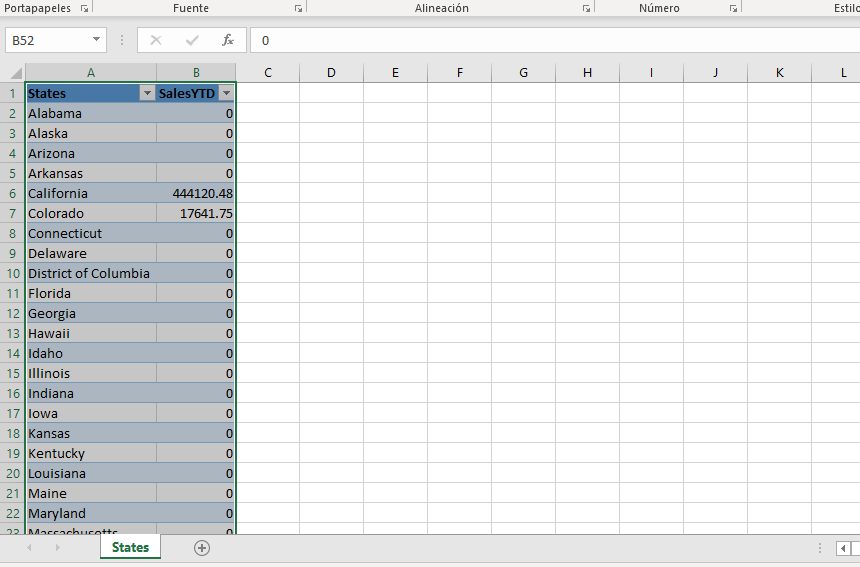
\includegraphics[width=15cm]{./Imagenes/EJER1T3(2)}
	\end{center}	

	\begin{center}
	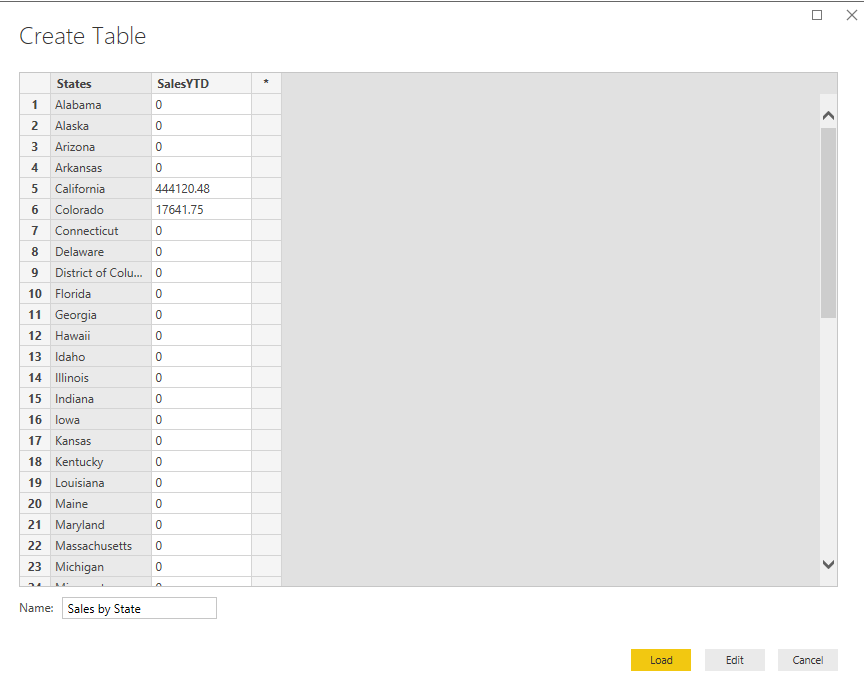
\includegraphics[width=15cm]{./Imagenes/EJER1T3(3)}
	\end{center}	

	\begin{center}
	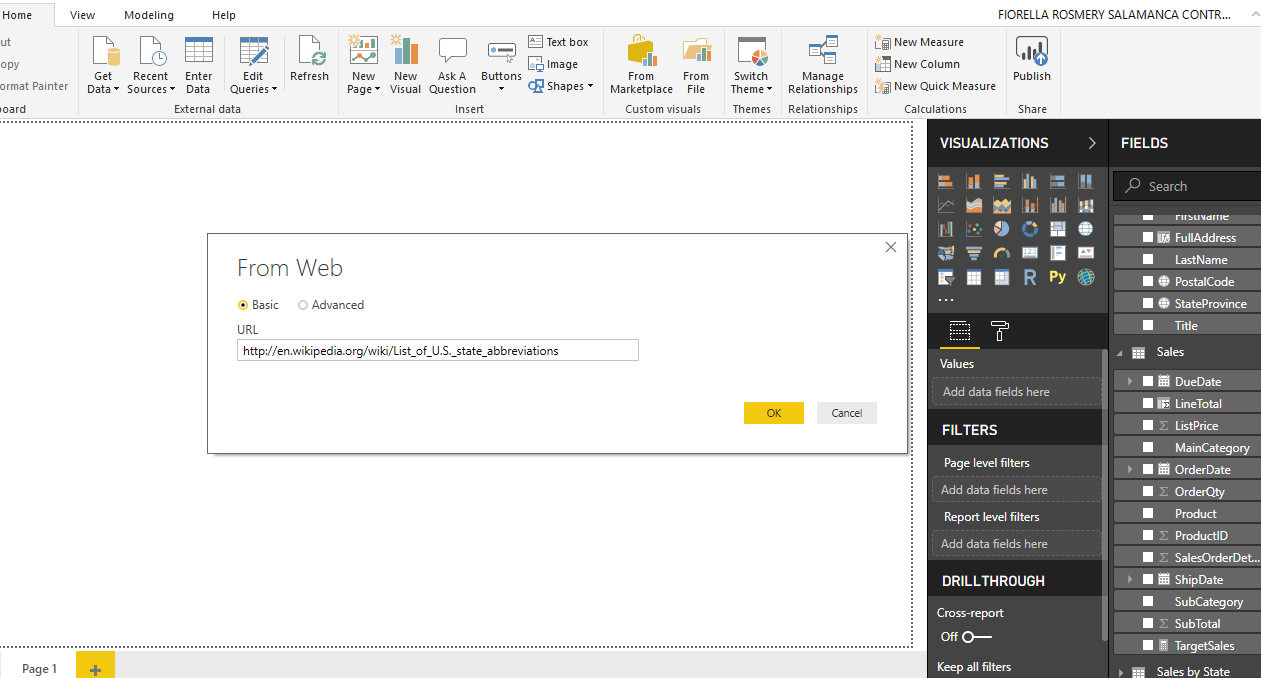
\includegraphics[width=15cm]{./Imagenes/EJER1T3(4)}
	\end{center}	

	\begin{center}
	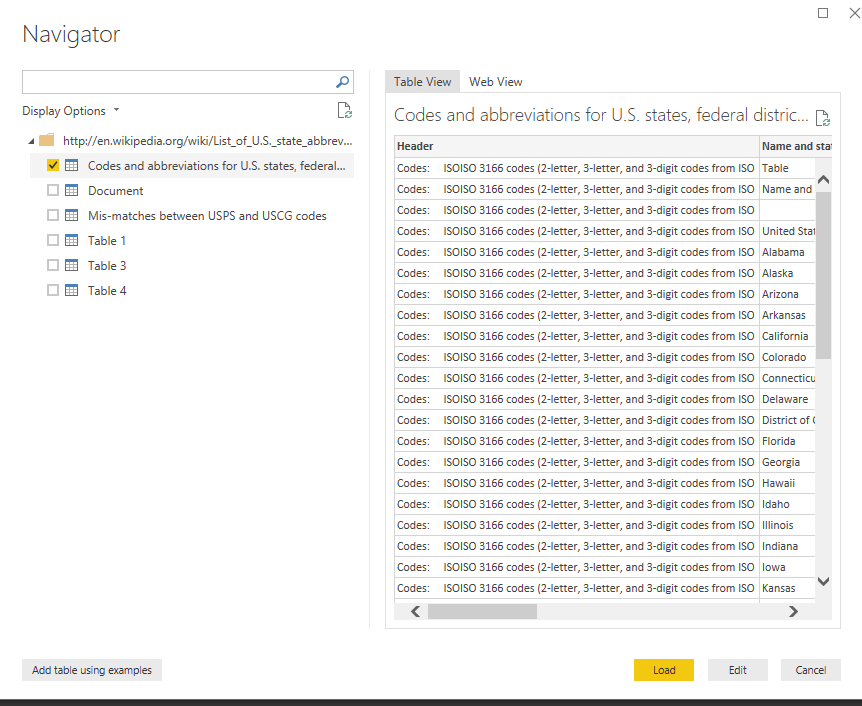
\includegraphics[width=15cm]{./Imagenes/EJER1T3(5)}
	\end{center}	

	\begin{center}
	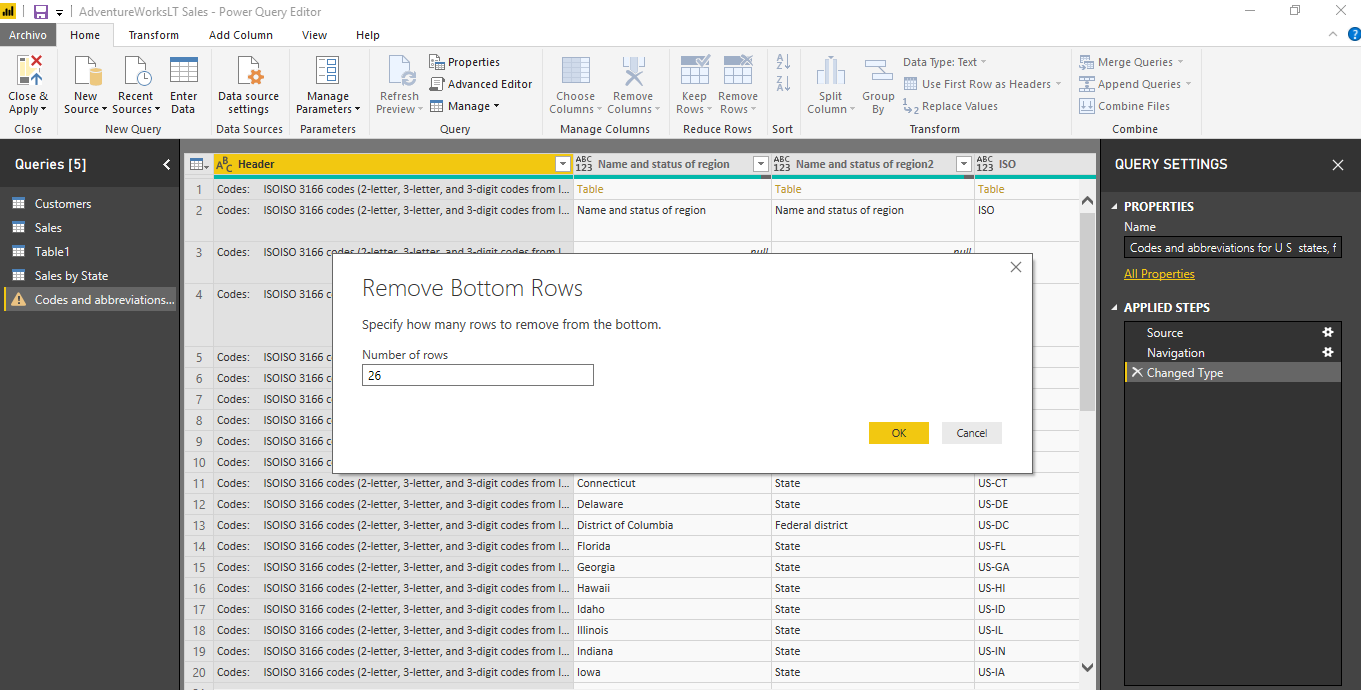
\includegraphics[width=15cm]{./Imagenes/EJER1T3(6)}
	\end{center}	

	\begin{center}
	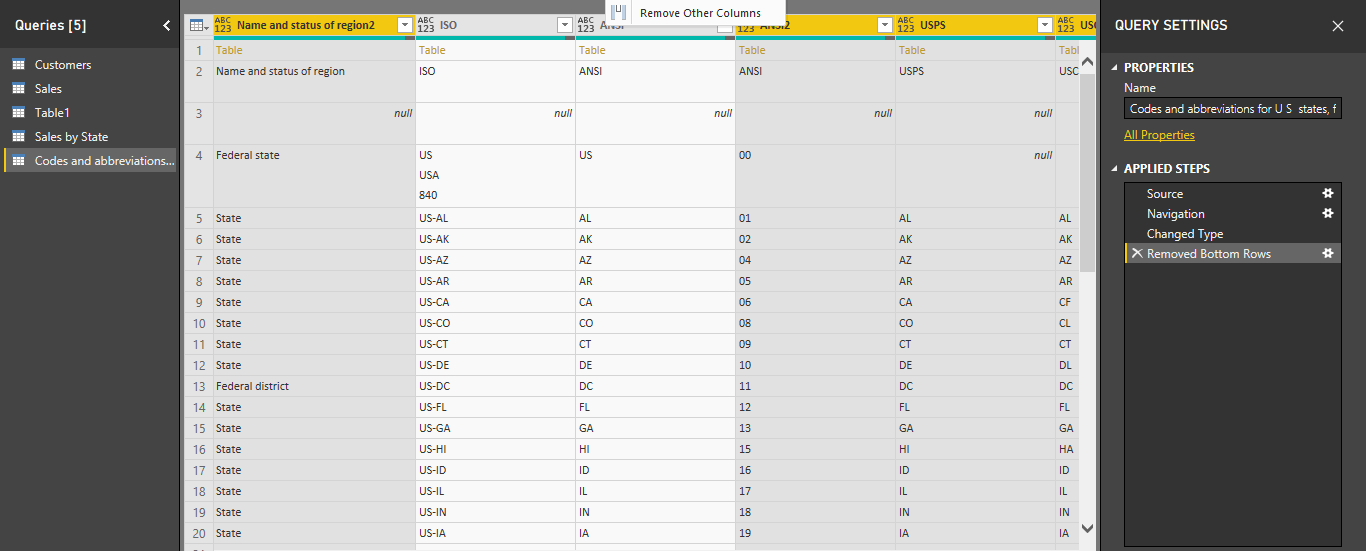
\includegraphics[width=15cm]{./Imagenes/EJER1T3(7)}
	\end{center}	

	\begin{center}
	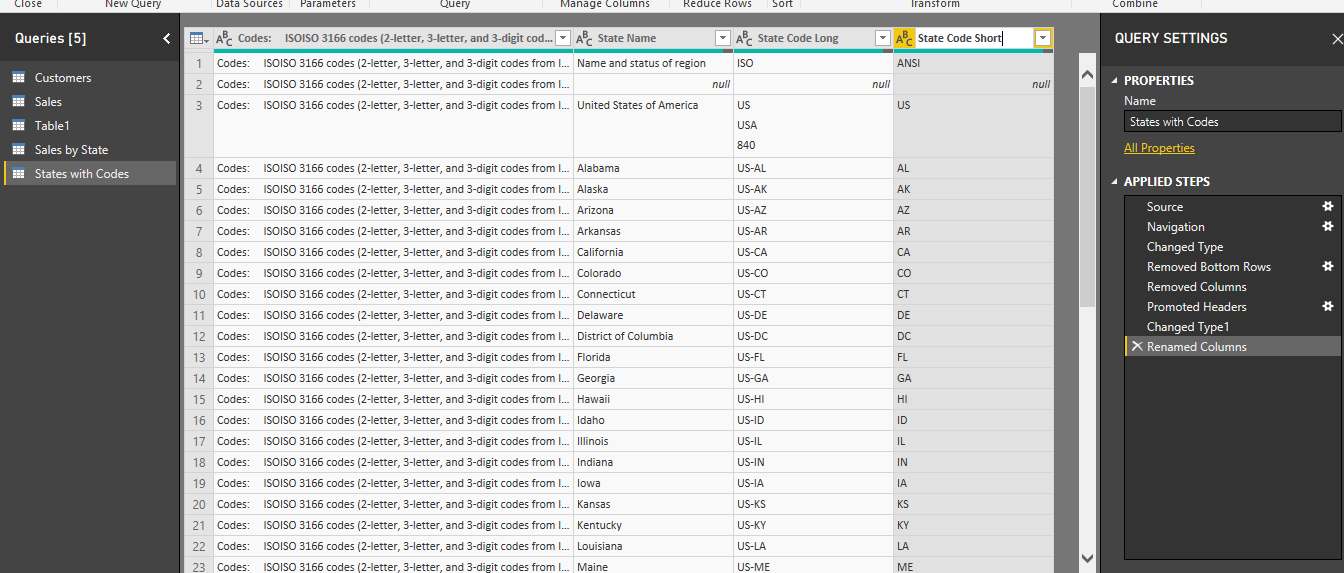
\includegraphics[width=15cm]{./Imagenes/EJER1T3(8)}
	\end{center}	

	\begin{center}
	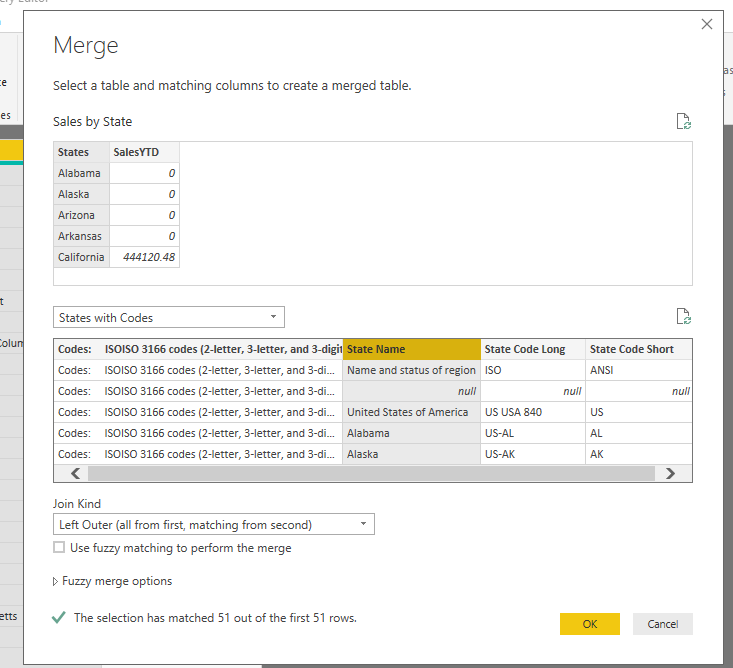
\includegraphics[width=15cm]{./Imagenes/EJER1T3(9)}
	\end{center}	



\section{Actividad No 01 – DESARROLLO} 

Ejercicio 1: Crear relaciones \\
Ejercicio 2: Cálculos \\

	\begin{center}
	\includegraphics[width=15cm]{./Imagenes/ley1}
	\end{center}	

	\begin{center}
	\includegraphics[width=15cm]{./Imagenes/ley2}
	\end{center}	

	\begin{center}
	\includegraphics[width=15cm]{./Imagenes/ley3}
	\end{center}	

	\begin{center}
	\includegraphics[width=15cm]{./Imagenes/ley4}
	\end{center}	

	\begin{center}
	\includegraphics[width=15cm]{./Imagenes/ley5}
	\end{center}	

	\begin{center}
	\includegraphics[width=15cm]{./Imagenes/ley6}
	\end{center}	

	\begin{center}
	\includegraphics[width=15cm]{./Imagenes/ley7}
	\end{center}	

	\begin{center}
	\includegraphics[width=15cm]{./Imagenes/ley8}
	\end{center}	

\section{Actividad No 01 – DESARROLLO} 

Ejercicio 1: Crear relaciones \\
Ejercicio 2: Cálculos \\

	\begin{center}
	\includegraphics[width=15cm]{./Imagenes/ley1}
	\end{center}	

	\begin{center}
	\includegraphics[width=15cm]{./Imagenes/ley2}
	\end{center}	

	\begin{center}
	\includegraphics[width=15cm]{./Imagenes/ley3}
	\end{center}	

	\begin{center}
	\includegraphics[width=15cm]{./Imagenes/ley4}
	\end{center}	

	\begin{center}
	\includegraphics[width=15cm]{./Imagenes/ley5}
	\end{center}	

	\begin{center}
	\includegraphics[width=15cm]{./Imagenes/ley6}
	\end{center}	

	\begin{center}
	\includegraphics[width=15cm]{./Imagenes/ley7}
	\end{center}	

	\begin{center}
	\includegraphics[width=15cm]{./Imagenes/ley8}
	\end{center}	


\end{document}
